\subsubsection{Testing the MQ6 gas sensor}
\par Next, we wanted to test this sensor independently. To do this we first started off with reading the data-sheet to find out the appropriate voltage input and pin layout. We found out that it operates at 5 volts with a minimum of 0 volts. We supplied 5 volts from the power supply to our breadboard and we used an LED to our output pin to see if it detects any gas. 
\begin{figure}[h!]
	\centering
	\begin{subfigure}[t]{0.45\textwidth}
		\centering
		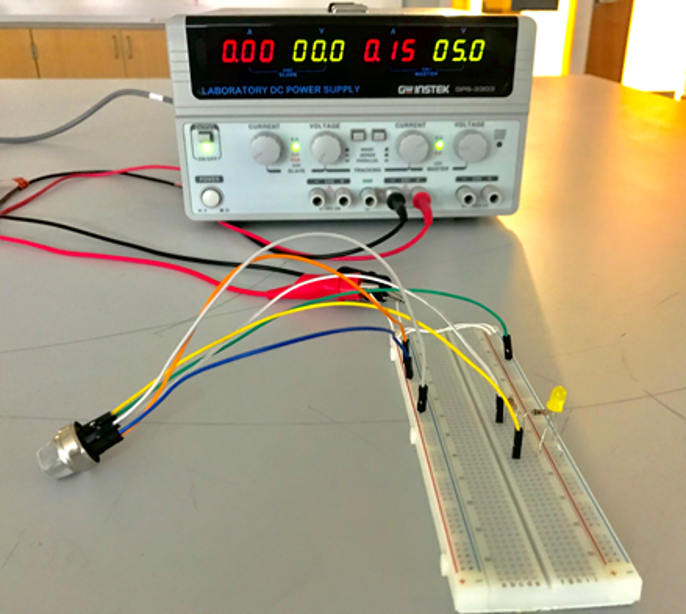
\includegraphics[height=1.5in]{mq6Test.png}
		\caption{LED on via pin 18}
	\end{subfigure}
	\begin{subfigure}[t]{0.45\textwidth}
		\centering
		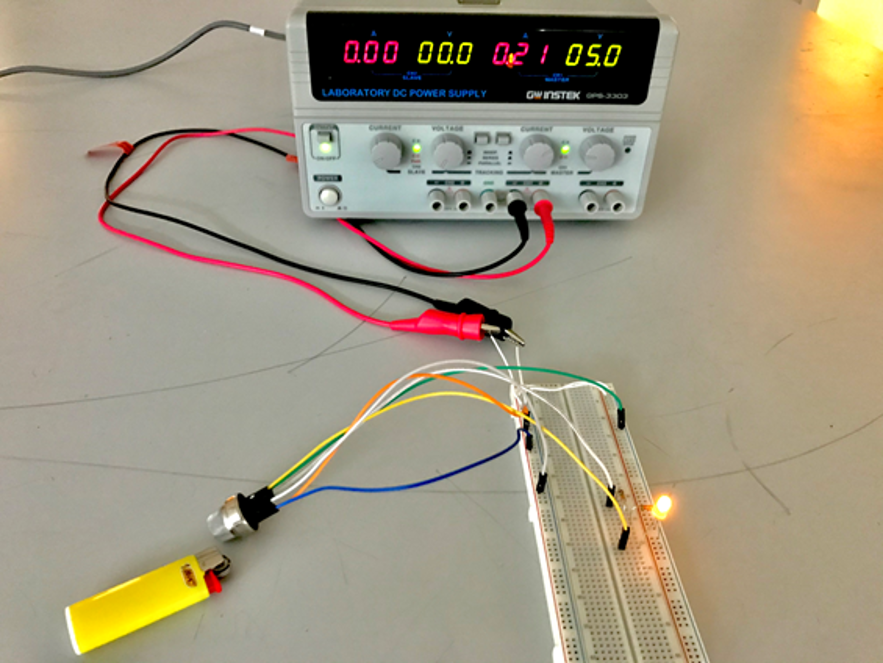
\includegraphics[height=1.5in]{mq6TestOn.png}
		\caption{LED off via pin 18}
	\end{subfigure}
	\caption{Simple LED activation over 802.15.4 (2)}
\end{figure}
\par Properly connected, the gas sensor produced quantifiable results. Using a common butane lighter, we tested the sensors ability to detect ambient gases. The LED was able to indicate the presence of LPG, thus we now know our gas sensing components are functional.
\par Since the XBee modules analog to digital converter requires an input in the range of 1.2 volts, we must reduce the 5 volt output of the gas sensor down to this level to be quantified and processed. To do this a simple voltage divider was designed (1). With voltages constant and one resistor value constant we only need to solve for one unknown (2).
\begin{equation}
V\textsubscript{out}=\frac{R1}{R1+R2}*V\textsubscript{in}
\end{equation}
Solving for R1: \\
\begin{equation}
1.2 = \frac{5100}{R1+5100}*5
\end{equation}
\[R1 = 16150 \Omega\]

% Testing the PIR Motion sensor
\subsubsection{Testing the PIR Motion Sensor}
\par The Parallax sensor allows us to choose between two set sensitivity levels, either an approximate range of 15 feet or 30 feet. This setting is changed with the manual moving of a jumper that connects a center pin with a second pin either on its left or right. In essence this is a crude switch. To yield as flexible a system as possible, a small DIP switch has been designed to toggle this setting. This allows the user to decide between a "Closer" or "Farther" setting depending on which is best suited to their operating environment. This would be set to the "Closer" option by default. 